\clearpage\section{Chapter 2: Structures}
The examples in the previous chapter employed data types whose values
are \textit{immutable}. For example, all operations that manipulate
numbers and strings compute new values, rather than modify existing
values. This chapter presents structured types that organize and store
collections of arbitrary (and possibly mixed) types of values. When you
complete this chapter, you will understand how to use these types.


\begin{itemize}
\item Tables associate their elements with key values for rapid lookup.
\item Lists offer efficient access by position as well as by
\index{stack}stack or \index{queue}queue operations.
\item Records store values using a fixed number of named fields.
\item Sets support operations such as union and intersection on groups
of elements.
\item Using structures to represent \index{tree}trees, graphs, and
matrices.
\end{itemize}
There are several structure types that describe different basic
relationships between values. The philosophy of structures in Unicon is
to provide built-in operators and functions for common organization and
access patterns - the flexible {\textquotedbl}super glue{\textquotedbl}
that is needed by nearly all applications. Their functionality is
similar to the C++ Standard Template Library or generic classes in
other languages, but Unicon{\textquotesingle}s structure types are much
simpler to learn and use, and are well supported by the expression
evaluation mechanism described in the previous chapter.

All structure types in Icon share many aspects in common, such as the
fact that structures are \index{mutable values}\textit{mutable}. The
values inside them may change. In that respect, structures are similar
to a collection of variables that are bundled together. In many cases,
Unicon{\textquotesingle}s structure types are almost interchangeable!
Operators like subscripts and built-in functions such as
\index{insert()}\textsf{insert()}\texttt{ }are defined consistently for
many types. Code that relies on such operators is
\index{polymorphism}\textit{polymorphic}: it may be used with multiple
structure types in an interchangeable way.

For both the structures described in this chapter and the strings
described in the next chapter, be aware that Unicon performs
\index{automatic storage management}automatic storage management, also
known as \index{garbage collection}garbage collection. If you have used
a language like C or C++, you know that one of the biggest headaches in
writing programs in these languages is tracking down bugs caused by
\index{memory allocation}memory allocation, especially dynamic heap
memory allocation. Unicon transparently takes care of those issues for
you.

Another big source of bugs in languages like C and C++ are
\index{pointer}pointers, values that contain raw \index{memory
addresses}memory addresses. Used properly, pointers are powerful and
efficient. The problem is that they are easy to use incorrectly by
accident; this is true for students and practicing software engineers
alike. It is easy in C to point at something that is off-limits, or to
trash some data through a pointer of the wrong type.

Unicon has no pointer types. Instead, all structure values implicitly
use pointer semantics. A \index{reference}\textit{reference} is a
pointer for which type information is maintained and type safety is
strictly enforced. In Icon, all structure values are references to
structure data that is allocated elsewhere, in a memory region known as
the heap. If you are a C programmer, think of a reference as a safe
pointer: the only operations it supports are copying the pointer, or
dereferencing it using an operation that is defined for its type.

Assigning a structure to a \index{variable}variable, or passing it as a
\index{parameter}parameter, gives that variable or parameter a copy of
the reference to the structure but does not make a copy of the
structure. If you want a copy of a structure, you call the function
\textsf{copy(x)}, which makes a {\textquotedbl}shallow{\textquotedbl}
copy of a single table, list, record, or set. If that structure
contains references to other structures as its elements, those
substructures are not copied by \textsf{copy()}. To copy a
{\textquotedbl}deep{\textquotedbl} structure (lists of lists, tables of
records, etc.) you can use the procedure \textsf{deepcopy()} that is
given as an example later in this chapter.

\subsection{Tables}
\index{table data type}Tables are unordered collections of values that
are accessed using \index{associative memory}associated \index{keys,
table}\textit{keys}. They are Unicon{\textquotesingle}s most versatile
type. All of the other structure types can be viewed as special cases
of tables, optimized for performance on common operations. Most
operations that are defined for tables are defined for other structure
types as well.

\index{table lookup}Subscripts are used for the primary operations of
associating keys with values that are inserted into the table, and then
using keys to look up objects in the table. The \textsf{table()}
function creates a new empty table. For example, the lines

\iconcode{
T := table() \\
T[{\textquotedbl}hello{\textquotedbl}] :=
{\textquotedbl}goodbye{\textquotedbl}
}

\noindent
create a new table, and associate the key
\textsf{{\textquotedbl}hello{\textquotedbl}} with the value
\textsf{{\textquotedbl}goodbye{\textquotedbl}}. The \textsf{table()}
function takes one optional argument: the \index{default
value!table}default value to return when lookup \index{expression
failure}fails. The default value of the default value is
\textsf{\&null}, so after the above example,
\textsf{write(T[{\textquotedbl}goodbye{\textquotedbl}])} would write an
empty line, since \textsf{write()} treats a null argument the same as
an empty string, and \textsf{write()} always writes a newline.
Assigning a value to a key that is not in the table inserts a value
into the table. This occurs in the second line of the example above, so
\ \textsf{write(T[{\textquotedbl}hello{\textquotedbl}])} writes out
\textsf{{\textquotedbl}goodbye{\textquotedbl}}.

Subscripts are the primary operation on tables, but there are several
other useful operations. The \index{insert()!table}\textsf{insert(T,
k}\textsf{\textsubscript{1}}\textsf{,
x}\textsf{\textsubscript{1}}\textsf{,
k}\textsf{\textsubscript{2}}\textsf{,
x}\textsf{\textsubscript{2}}\textsf{, ...)} function adds new key-value
pairs to \textsf{T}. The \index{delete()!table}\textsf{delete(T,
k}\textsf{\textsubscript{1}}\textsf{,
k}\textsf{\textsubscript{2}}\textsf{, ...)} function deletes values
from \textsf{T} that correspond to the supplied keys.
Icon{\textquotesingle}s unary \textsf{*} operator produces the size of
its argument; for a table, \index{table!length *T}\textsf{*T} is the
number of key-value pairs in the table. Unary \textsf{!} generates
elements from a collection; for a table, \textsf{!T} generates the
values stored in the table. Unary \textsf{?} is the random operator;
for a table, \textsf{?T} produces a random value stored in the table.
Both unary \textsf{!} and \textsf{?} produce values stored in a table,
not the keys used to lookup values.

Function \index{member()!table}\textsf{member(T, k)} succeeds if
\textsf{k} is a key in \textsf{T} and fails otherwise. Function
\index{key()!table}\textsf{key(T)} generates the keys with which values
have been stored. Here is a code fragment to print a word count of the
input (assuming the \textsf{getword()} procedure generates words of
interest): 

\iconcode{
wordcount := table(0) \\
every word := getword() do wordcount[word] +:= 1 \\
every word := key(wordcount) do write(word, {\textquotedbl}
\ {\textquotedbl}, wordcount[word])
}

The default value for the table is 0. When a new word is inserted, the
default value gets incremented and the new value (that is, 1) is stored
with the new word. Tables grow automatically as new elements are
inserted.

\subsection[Lists]{Lists}
\index{list data type}Lists are ubiquitous dynamically sized ordered
collections of values. They are accessed using subscripts, with indexes
starting at 1. You can also modify lists by inserting or removing
elements from the beginning, middle, or end of the list. Lists take the
place of \index{array}arrays, \index{stack}stacks, \index{queue}queues,
and \index{deque}deques found in other languages and data structures
textbooks.

A list is created by calling the function \index{list()}\textsf{list()},
which takes optional parameters for the lists{\textquotesingle}s
initial size and the initial value given to all elements of the list.
By default \textsf{list()} creates an empty list. Alternatively, you
can create a list by enclosing a comma-separated sequence of values in
square brackets: 

\iconcode{
L := [{\textquotedbl}linux{\textquotedbl}, 2.0,
	{\textquotedbl}unix{\textquotedbl}]
}

Lists are dynamic. \index{insert()!list}\textsf{insert(L, i, x)} inserts
\textsf{x} at position \textsf{i}, and
\index{delete()!list}\textsf{delete(L, i)}\texttt{ }deletes the element
at position \textsf{i}. In addition, lists grow or shrink as a result
of stack and queue operations. The \index{push()}\textsf{push()} and
\index{pop()}\textsf{pop()} functions add and remove elements from the
front of a list, while \index{put()}\textsf{put()} and
\index{pull(L)}\textsf{pull()} add and remove elements at the end of
the list. The previous list could have been constructed one element at
a time with the following code. The expression \textsf{[]} is another
way to create an \index{empty list}empty list; it is equivalent to
calling \textsf{list()} with no arguments.

\iconcode{
L := [ ] \\
put(L, {\textquotedbl}linux{\textquotedbl}) \\
put(L, 2.0) \\
put(L, {\textquotedbl}unix{\textquotedbl})
}

Elements of the list can be obtained either through list manipulation
functions or by subscripting. Given the list \textsf{L} above, in the
following code the first line writes
\textsf{{\textquotedbl}unix{\textquotedbl}} while the second line moves
the first element to the end of the list.

\iconcode{
write(L[3]) \\
put(L, pop(L))
}

There is no restriction on the kinds of values that may be stored in a
list. For example, the elements of a list can themselves be lists. You
can create lists like

\iconcode{
L := [[1, 2, 3], [4, 5, 6], [7, 8, 9]]}

\noindent and index them with multiple subscripts. \textsf{L[2][3]} is
equivalent to \textsf{L[2,3]} and yields the value 6 in this example. 

Lists also support several common operators. The operator
\index{list!size (*L)}\textsf{*L} produces the size of list \textsf{L}.
The operators \textsf{!L} and \textsf{?L} generate the elements of
\textsf{L} in sequence, and produce a single random element of
\textsf{L}, respectively. The following procedure uses the unary
\textsf{!} operator to sum the values in list \textsf{L}, which must be
numbers.

\iconcode{
procedure sum(L) \\
\>   total := 0 \\
\>   every total +:= !L \\
\>   return total \\
end
}

Comparing the two, lists are like tables with really boring keys, the
positive integers starting from 1. Function \textsf{member(L, k)}
succeeds if \textsf{0 {\textless} integer(k) {\textless}= *L}, while
\textsf{key(L)} is equivalent to the expression \textsf{1 to *L}. List
indexes are contiguous, unlike table keys, and so lists can support a
\index{slice!list L[i:j]}\textit{slice} operator to produce a sublist,
given a pair of indexes to mark the bounds. The \textsf{L[i:j]}
expression produces a new list that contains a copy of the elements in
\textsf{L} between positions \textsf{i} and \textsf{j}. The
\textsf{L[i+:j]} expression is equivalent to \textsf{L[i:i+j]}. List
concatenation is another valuable operator. The \index{list
concatenation!L1 {\textbar}{\textbar}{\textbar} L2}\textsf{L1
{\textbar}{\textbar}{\textbar} L2} expression produces a new list whose
elements are a copy of the elements in \textsf{L1} followed by a copy
of the elements in \textsf{L2}.

\subsection{Records}
A \index{record}record is a fixed-sized, ordered collection of values
whose elements are accessed using user-defined named \textit{fields}. A
record is declared as a global name that introduces a new type with a
corresponding \index{constructor!record}constructor procedure, as in
the following example. The field names are a comma-separated list of
identifiers enclosed in parentheses.

\iconcode{
record complex(re, im)}

Record \index{instance!record}\textit{instances} are created using a
constructor procedure with the name of the record type. On such
instances, fields are accessed by name using a dot notation or string
subscript, or by integer index subscript. The upshot of all this is
that you can use records as records, or as special tables or lists with
a constant size and fixed set of keys.

\textsf{member(R,s)} tests whether \textsf{s} is a field in \textsf{R};
\textsf{key(R)} generates \textsf{R}{\textquotesingle}s field names.
Functions like \textsf{insert()}, or \textsf{push()} are not supported
on records, since they change the size of the structure that they
modify. Here is a demonstration of record operations.

\iconcode{
a := complex(0, 0) \\
b := complex(1, -1) \\
if a.re = b.re then write({\textquotedbl}not likely{\textquotedbl}) \\
if a[{\textquotedbl}re{\textquotedbl}] = a[2] then
write({\textquotedbl}a.re and a.im are equal{\textquotedbl})
}

Unicon provides a mechanism for constructing new record types on the
fly, described in Chapter 6, as well as the ability to declare classes,
which are new data types that form the building blocks for
object-oriented programs, described starting in Chapter 8. Records are
closely related to classes and objects: they can be considered to be an
optimized special case of objects that have no methods. \ 

\subsection{Sets}

A \index{set data type}set is an unordered collection of values with the
uniqueness property: an element can only be present in a set once. The
function \textsf{set(x...)} creates a set containing its arguments. For
the sake of backward compatibility with Icon, list arguments to
\textsf{set()} are not inserted; instead, the list elements are
inserted. As with other structures, the elements may be of any type,
and may be mixed. For example, the assignment

\iconcode{
S := set({\textquotedbl}rock lobster{\textquotedbl},
{\textquotesingle}B{\textquotesingle}, 52)}

\noindent
creates a set with three members: a string, a cset, and an integer. \ An
equivalent set is constructed by the call
\textsf{set([{\textquotedbl}rock lobster{\textquotedbl},
{\textquotesingle}B{\textquotesingle}, 52])}. \ If you want a list as a
member of a set, wrap it inside another list, as in \textsf{set([L])},
or insert the list into the set after it is created.

The functions \index{member()!set}\textsf{member()},
\index{insert()!set}\textsf{insert()}, and
\index{delete()!set}\textsf{delete()} do what their names suggest. As
for csets in the previous chapter, \index{union
(S1++S2)}\textsf{S1++S2}, \index{intersection (S1**S2)}\textsf{S1**S2},
and \index{difference (S1-{}-S2)}\textsf{S1-{}-S2} are the union,
intersection, and difference of sets \textsf{S1} and \textsf{S2}. Set
operators construct new sets and do not modify their operands. Because
a set can contain any value, it can contain a
\index{reference}reference to itself. This is one of several
differences between Unicon sets, which are mutable structures, and
mathematical sets. Another difference is that Unicon sets have a finite
number of elements, while mathematical sets can be infinite in size.

As a short example, consider the following program, called
\textsf{uniq}, that filters duplicate lines in its standard input as it
writes to its standard output. Unlike the UNIX utility of this name,
our version does not require the duplicate lines to be adjacent.

\iconcode{
procedure main() \\
\>   S := set() \\
\>   while line := read() do \\
\>   \ \ \ if not member(S, line) then \{ \\
\>   \ \ \ \ \ \ insert(S, line) \\
\>   \ \ \ \ \ \ write(line) \\
\>   \ \ \ \ \ \ \} \\
end
}

Sets are closely related to the table data type. They are very similar
to an optimized special case of tables that map all keys to the value
\textsf{\&null}. Unlike tables, sets have no default value and do not
support the \index{subscript operator}subscript operator.

\subsection{Using Structures}
The elements of structures can be other structures, allowing you to
organize information in whatever way best fits your application. In
Unicon building complex structures such as a table of lists, or a list
of records that contain sets, requires no special trickery or new
syntax. A few examples of how such structures are accessed and
traversed will get you started. \index{recursion}Recursion is often
involved in operations on complex structures, so it plays a prominent
role in our examples. The concept of recursion was discussed in Chapter
1.

\subsubsection{A Deep Copy}
The built-in function \index{copy(x)}\textsf{copy(x)} makes a one-level
copy of structure values. For a multi-level structure, you need to call
\textsf{copy()} for each substructure if the new structure must not
\index{pointer}point into the old structure. This is a natural task for
a recursive function.

\iconcode{
procedure deepcopy(x) \\
\>   local y \\
\>   case type(x) of \{ \\
\>   {\textquotedbl}table{\textquotedbl}{\textbar}{\textquotedbl}list{\textquotedbl}{\textbar}{\textquotedbl}record{\textquotedbl}: \{ \\
\>   \ \ \ y := copy(x) \\
\>   \ \ \ every k := key(x) do y[k] := deepcopy(x[k]) \\
\>   \ \ \ \} \\
\>   {\textquotedbl}set{\textquotedbl}: \{ \\
\>   \ \ \ y := set() \\
\>   \ \ \ every insert(y, deepcopy(!x)) \\
\>   \ \ \ \} \\
\>   default: return x \\
\>   \} \\
\>   return y \\
end
}

This version of \index{deepcopy()}\textsf{deepcopy()} works for
arbitrarily deep \index{tree}tree structures, but the program execution
will crash if \textsf{deepcopy()} is called on a structure containing
cycles. It also does not copy directed acyclic graphs correctly. In
both cases the problem is one of not noticing when you have already
copied a structure, and copying it again. The Icon Program Library has
a deep copy procedure that handles this problem, and we present the
general technique that is used to solve it in the next section.

\subsubsection{Representing Trees and Graphs}
Since there is no restriction on the types of values in a list, they can
be other lists too. Here is an example of how a tree may be implemented
with records and lists:

\iconcode{
record node(name, links) \\
\>   ... \\
barney := node({\textquotedbl}Barney{\textquotedbl}, list()) \\
betty := node({\textquotedbl}Betty{\textquotedbl}, list()) \\
bambam := node({\textquotedbl}Bam-Bam{\textquotedbl}, [barney, betty])
}

The structure created by these expressions is depicted in Figure 2-1.
The list of links at each node allows trees with an arbitrary number of
children at the cost of extra memory and indirection in the tree
traversals. The same representation works for arbitrary
\index{graph}graphs.



\begin{center}
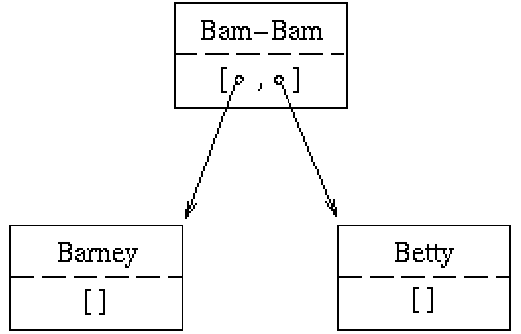
\includegraphics[width=3in,height=1.9in]{ub-img/ub-img6.png}
\end{center}

{\sffamily\bfseries Figure 2-1:}
{\sffamily A Record Containing a List of Two Records}

\bigskip

To find every node related to variable \textsf{bambam}, follow all the
links reachable starting from \textsf{bambam}. Here is a procedure that
performs this task.

\iconcode{
procedure print\_relatives(n) \\
local i \\
static relatives \\
initial relatives := set() \\
every i := n {\textbar} !n.links do \{  \\
\>   \ \ \ if not member(relatives, i.name) then \{  \\
\>   \ \ \ \ \ \ write(i.name) \\
\>   \ \ \ \ \ \ insert(relatives, i.name) \\
\>   \ \ \ \ \ \ print\_relatives(i) \\
\>   \ \ \ \ \ \ \} \\
\>   \ \ \ \} \\
end
}

Calling print\_relatives(bambam) will print

\iconcode{
Bam-Bam\\
Barney\\
Betty
}

Static variables and the \textsf{initial} clause are explained in
Chapter 1. Can you guess what purpose \index{static}static variable
\textsf{relatives} serves? For a proper tree structure, it is not
needed at all, but for more general data structures such as directed
graphs this static variable is very important! One defect of this
procedure is that there is no way to reset the static variable and call
\textsf{print\_relatives()} starting from scratch. How would you remove
this defect?

\subsubsection[The n{}-Queens Example]{The \textit{n}{}-Queens Example}
The \index{8-Queens problem}8-Queens problem is a classic
\index{backtracking}backtracking problem. The goal is to place eight
queens on a chessboard so that none of the queens attack any other.
Here is a solution to a more general form of the problem, that of
placing \index{n queens}\textit{n} queens on an \textit{n} \textsf{x}
\textit{n} board. The solution we present is by Steve \index{Wampler,
Steve}Wampler, and it is in the Icon Program Library.

An array of size \textsf{n} stores the solutions, with each element
representing a column. The values in the array are integers specifying
the row in each column that has the queen. (Since the queens cannot
attack each other, each column must contain exactly one queen.) The
problem size \textsf{n} and the array are declared \textsf{global} so
that all procedures can see them; this allows the program to avoid
passing these variables in to every procedure call. Use globals
sparingly, and only where they are appropriate, as is the case here.

\iconcode{
link options \\
global solution, n \\
procedure main(args) \\
local i, opts
}

The program starts by handling command-line arguments. In Unicon
programs, \textsf{main()} is called with a single parameter that is a
list of strings whose elements are the command-line arguments of the
program.

The n-queens program recognizes only one thing on the command line: the
option \textsf{{}-n} followed by an integer specifies the size of board
to use. Thus the command line \textsf{queens -n 9} will generate
solutions on a 9x9 board. The default value of \textsf{n} is 6. The
\index{options()}\textsf{options()} procedure is an Icon Program
Library procedure described in Appendix B; it removes options from the
command line and places them in a table whose keys are option letters
such as \textsf{{\textquotedbl}n{\textquotedbl}}. Library procedures
such as \textsf{options()} are incorporated into a program using the
\index{link}\textsf{link} declaration, as in the \textsf{link options}
that begins the code fragment above. A link declaration adds the
procedures, global variables, and record types in the named module (in
this case, procedure \textsf{options()} came from a file
\textsf{options.icn}) to the program.

\iconcode{
\>   opts := options(args,{\textquotedbl}n+{\textquotedbl}) \\
\>   n := {\textbackslash}opts[{\textquotedbl}n{\textquotedbl}]
{\textbar} 6 \\
\>   if n {\textless}= 0 then stop({\textquotedbl}-n needs a positive
numeric parameter{\textquotedbl})
}

The value \textsf{n} gives the size for the solution array and also
appears in a banner:

\iconcode{
\>   solution := list(n) \ \ \# a list of column solutions \\
\>   write(n,{\textquotedbl}-Queens:{\textquotedbl}) \\
\>   every q(1) \ \ \ \ \ \ \ \ \ \ \ \# start by placing queen in
first column \\
end
}

Now comes the meat of the program, the procedure \textsf{q(c)}. It tries
to place a queen in column \textsf{c} and then calls itself recursively
to place queens in the column to the right. The \textsf{q(c)} procedure
uses three arrays: \textsf{rows}, \textsf{up}, \ and \textsf{down}.
They are declared to be \textit{static}, meaning that their values will
be preserved between executions of the procedure, and all
\index{instance}instances of the procedure will share the same lists.
Since each row must have exactly one queen, the rows array helps to
make sure any queen that is placed is not on a row that already has a
queen. The other two arrays handle the diagonals: \textsf{up} is an
array (of size \textit{2n-1}) of the upward slanting diagonals, and
\textsf{down} is an array for the downward slanting diagonals. Two
queens in positions \textit{(r\_1, c\_1)} and \textit{(r\_2, c\_2)} are
on the same {\textquotedbl}up{\textquotedbl} diagonal if
\textit{n+r\_1-c\_1 = n+r\_2-c\_2} and they are on the same
{\textquotedbl}down{\textquotedbl} diagonal if \textit{r\_1+c\_1-1 =
r\_2+c\_2-1}. Figure 2-2 shows some of the
{\textquotedbl}up{\textquotedbl} and {\textquotedbl}down{\textquotedbl}
diagonals.

\bigskip

\begin{center}
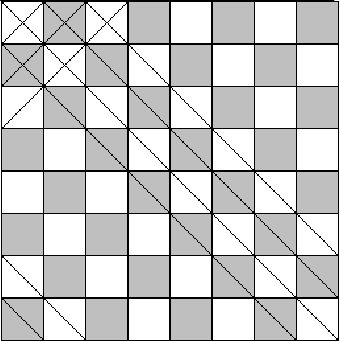
\includegraphics[width=3.5in,height=3.5in]{ub-img/diagonal.png}
\end{center}
{\sffamily\bfseries Figure 2-2:}
{\sffamily Up and Down Diagonals in the n-Queens Problem}

\bigskip

\iconcode{
\# \\
\# q(c) - place a queen in column c. \\
\# \\
procedure q(c) \\
local r \\
static up, down, rows \\
initial \{ \\
\>   up := list(2*n-1,0) \\
\>   down := list(2*n-1,0) \\
\>   rows := list(n,0) \\
\>   \}
}

The next expression in \textsf{q()} is an \textsf{every} loop that tries
all possible values for the queen in row \textsf{c}. The variable
\textsf{r} steps through rows 1 to 8. For any row at which the program
places a queen, it must ensure that

1.\ \ \textsf{rows[r]} is zero, that is, no other column has a queen in
row \textsf{r}\textsf{,}

2.\ \ \textsf{up[n+r-c]} is 0, that is, there is not already a queen in
the {\textquotedbl}up{\textquotedbl} diagonal, and

3.\ \ \textsf{down[r+c-1]} is 0, that is, there is not already a queen
in the down diagonal.

If these conditions are met, then it is OK to place a queen by assigning
a 1 to all those arrays in the appropriate position:

\iconcode{
\>   every 0 = rows[r := 1 to n] = up[n+r-c] = down[r+c-1] \& \\
\>   \ \ \ rows[r] {\textless}- up[n+r-c] {\textless}- down[r+c-1]
{\textless}- 1 do \{
}

For \index{assignment}assignment, instead of \textsf{:=} this expression
uses the \index{reversible assignment}\textit{reversible assignment}
operator \textsf{{\textless}-}. This assigns a value just like in
conventional assignment, but it remembers the old value; if it is ever
resumed, it restores the old value and \index{expression failure}fails.
This causes the appropriate entries in the \textsf{row},
\textsf{up}\texttt{,} and \textsf{down} arrays will be reinitialized
between iterations.

When the \textsf{every} loop found a good placement for this column,
either the program is done (if this was the last column) or else it is
time to try to place a queen in the next row:

\iconcode{
\>   \ \ \ solution[c] := r \ \ \ \ \ \ \# record placement. \\
\>   \ \ \ if c = n then show() \\
\>   \ \ \ else q(c + 1) \ \ \ \ \ \ \ \ \ \# try to place next queen. \\
\>   \ \ \ \} \\
end
}

That{\textquotesingle}s it! The rest of the program just prints out any
solutions that were found.

Printing the chess board is similar to other reports you might write
that need to create horizontal lines for tables. The \textsf{repl()}
function is handy for such situations. The \textsf{repl(s, i)} function
returns \textsf{i} {\textquotedbl}replicas{\textquotedbl} of string
\textsf{s} concatenated together. The \textsf{show()} function uses it
to create the chessboard.\textit{ }

\iconcode{
\# \\
\# show the solution on a chess board. \\
\# \\
procedure show() \\
static count, line, border \\
initial \{ \\
\>   count := 0 \\
\>   line := repl({\textquotedbl}{\textbar} \ \ {\textquotedbl},n)
{\textbar}{\textbar} {\textquotedbl}{\textbar}{\textquotedbl} \\
\>   border := repl({\textquotedbl}-{}-{}-{}-{\textquotedbl},n)
{\textbar}{\textbar} {\textquotedbl}-{\textquotedbl} \\
\>   \} \\
\>   write({\textquotedbl}solution: {\textquotedbl}, count+:=1,
{\textquotedbl}{\textbackslash}n \ {\textquotedbl}, border) \\
\>   every line[4*(!solution - 1) + 3] {\textless}-
{\textquotedbl}Q{\textquotedbl} do \{ \\
\>   \ \ \ write({\textquotedbl} \ {\textquotedbl}, line,
{\textquotedblleft}{\textbackslash}n \ {\textquotedbl}, border) \\
\>   \ \ \ \} \\
\>   write() \\
end
}

{\sffamily
Summary}

Unicon{\textquotesingle}s structures are better than sliced bread. To be
fair, this is because Icon{\textquotesingle}s inventors really got
things right. These structures are the foundations of complex
algorithms and the glue that builds sophisticated data models. They are
every computer scientists{\textquotesingle} buzzword-compliant best
friends: polymorphic, heterogeneous, implicitly referenced,
cycle-capable, dynamically represented, and automatically reclaimed.
They provide a direct implementation of the common information
associations used in object-oriented design. But most important of all,
they are extremely simple to learn and use.


\bigskip

\clearpage
\bigskip
